% $Id: examples.tex,v 1.13 2001-07-20 16:51:52 geuzaine Exp $

%
% WARNING:
%
% If \bigpictures is set to 1, the pictures must have been checked out
% (cvs module name is getdp-picts) in the ../../../getdp-picts directory.
%

% ---------------------------------------------------------------------------
\part{Examples}
% ---------------------------------------------------------------------------

\begin{slide}

\slidepagestyle{none}

\begin{center}
\bigtitle{Examples}\\
\ifnum\fulltitle=1\par\bigskip\bigskip
\mediumtitle{Patrick Dular and Christophe Geuzaine}\\
\bigskip
\smalltitle{Department of Electrical Engineering}\\
\smalltitle{Montefiore Institute B28, Sart Tilman Campus}\\
\smalltitle{University of Li�ge}\\
\smalltitle{B-4000 Li�ge (BELGIUM)}
\fi
\end{center}

\end{slide}

% ---------------------------------------------------------------------------

\chapter{Magnetostatics}

\ifnum\bigpictures=1

\begin{slide}

\begin{center}
\includegraphics[width=0.37\textwidth]{getdp-picts/ind1}%
\includegraphics[width=0.37\textwidth]{getdp-picts/ind2}

\includegraphics[width=0.37\textwidth]{getdp-picts/ind3}%
\includegraphics[width=0.37\textwidth]{getdp-picts/ind4}
\end{center}

\end{slide}

\fi

\begin{slide}

\mybox{colbox}{0.98\textwidth}{
\begin{equation*}
\Curl{\vec{h}} = \vec{j} ,\quad
\Div{\vec{b}} = 0 \quad\text{and}\quad
\vec{b} = \mu \vec{h} + \mu_0 \vec{h}_m 
\end{equation*}
\begin{equation*}
\begin{split}
\xymatrix{
 \color{colpos}\phi    \ar@{->}[r]^-{\GradSymb_h}  &
 \vec{h} \ar@{->}[r]^-{\CurlSymb_h} \ar@{<->}[d]^{\mu} &
 \vec{j} \ar@{->}[r]^-{\DivSymb_h}   &
 0 \\
 0       \ar@{<-}[r]^-{\DivSymb_e}&
 \vec{b} \ar@{<-}[r]^-{\CurlSymb_e}&
 \color{colpos}\vec{a} 
}
\end{split}
\end{equation*}
}

\begin{slideitemize}
\item Weak form of Gauss' law: 
\begin{equation*}
% \ivol{\Div{\vec{b}}}{\phi'} = 0 \Rightarrow
\ivol{\vec{b}}{\Grad{\phi'}} + \isur{\psca{\vec{n}}{\vec{b}}}{\phi'} 
= 0
\quad \forall\phi'\in\Hone[_0]{\Omega}
\end{equation*}

\item Weak form of Amp�re's law:
\begin{equation*}
% \ivol{\Curl{\vec{h}}}{\vec{a}'} = \ivol{\vec{j}}{\vec{a}'} \Rightarrow
\ivol{\vec{h}}{\Curl{\vec{a}'}} + \isur{\pvec{\vec{n}}{\vec{h}}}{\vec{a}'}
= \ivol{\vec{j}}{\vec{a}'} 
\quad \forall\vec{a}'\in\Hcurl[_0]{\Omega}
\end{equation*}

\end{slideitemize}

\end{slide}

% ---------------------------------------------------------------------------

\chapter{Magnetostatics: $\vec{b}$-conforming}

\begin{slide}

\mybox{colbox}{0.98\textwidth}{
\begin{center}
\emph{Vector potential} formulation
\begin{equation*}
\vec{b} = \Curl{\vec{a}}
\end{equation*}
\end{center}
}

\begin{center}
$\Downarrow$\\
Weak form of Amp�re's law\\
$\Downarrow$\\
$\displaystyle\ivol{\mu^{-1}\Curl{\vec{a}}}{\Curl{\vec{a}'}} 
= \ivol{\vec{j}}{\vec{a}'} ,
\quad\forall\vec{a}'\in\Hcurl[_0]{\Omega}$
\end{center}

\bigskip
NB: gauge for $\vec{a}$, ...

\end{slide}

\ifnum\bigpictures=1

\background{7\semcm}{0\semcm}{\includegraphics[width=0.38\textwidth]{getdp-picts/ind1}}

\fi

\begin{slide}

\begin{smallsyntax}
Group \{
  Core = #1; Inductor = #2; SkinInductor = #3, Air = #4;
  Omega = Region[\{Core, Inductor, Air\}];
\}
Function \{
  mu0 = 4.e-7 * Pi; mur = 1000;
  mu[ Core ] = mur * mu0;
  mu[ Region[\{Air, Inductor\}] ] = mu0;
  j[ Inductor ] = ...; //to be defined
\}
Constraint \{
  \{ Name a; 
    Case \{ 
      \{ Region CL_a0; Value 0; \}
    \}
  \}
\}
\end{smallsyntax}

\end{slide}

\background{}{}{}

\begin{slide}

\begin{smallsyntax}
FunctionSpace \{
  \{ Name Hcurl; Type Form1; \CC{vector potential}
    BasisFunction \{
      \{ Name se;  NameOfCoef ae; Function BF_Edge; Support Omega; 
        Entity EdgesOf[All]; \} \CC{associated with the edges of the mesh}
    \}
    Constraint \{ \CC{essential constraint + gauge (unicity)}
      \{ NameOfCoef ae;  EntityType EdgesOf; NameOfConstraint a; \}
      \{ NameOfCoef ae;  EntityType EdgesOfTreeIn;
        EntitySubType StartingOn; NameOfConstraint Gauge; \}
    \}
  \}
\}
\end{smallsyntax}

\end{slide}

\begin{slide}

\begin{smallsyntax}
Formulation \{
  \{ Name MagSta_a; Type FemEquation;
    Quantity \{ 
      \{ Name a; Type Local; NameOfSpace Hcurl; \}
    \}
    Equation \{
      Galerkin \{ [ 1/mu[] * Dof\{Curl a\} , \{Curl a\} ]; 
                 In Omega; Integration I1; Jacobian JVol; \}
      Galerkin \{ [ -j[] , \{a\} ]; 
                 In Inductor; Integration I1; Jacobian JVol; \}
    \}
  \}
\}
\end{smallsyntax}

\end{slide}

\begin{slide}

\begin{smallsyntax}
Resolution \{
  \{ Name MagSta_a;
    System \{
      \{ Name A; NameOfFormulation MagSta_a; \}
    \}
    Operation \{ Generate[A]; Solve[A]; SaveSolution[A]; \}
  \}
\}
PostProcessing \{
  \{ Name test; NameOfFormulation MagSta_a;
    Quantity \{
      \{ Name a; Value \{ Local\{ [ \{a\} ]; In Omega; \} \} \}
      \{ Name normb; Value \{ Local\{ [ Norm[\{d a\}] ]; Omega; \} \} \}
    \}
  \}
\}
\end{smallsyntax}

\end{slide}

\begin{slide}

Magnetodynamics?

Additional term in the formulation: 

\begin{smallsyntax}
      Galerkin \{ DtDof [ sigma[] * Dof\{a\} , \{a\} ]; 
                 In Core; Integration I1; Jacobian JVol; \}   
\end{smallsyntax}

New resolution:
\begin{smallsyntax}
  \{ Name MagDyn_a_t; \CC{time domain}
    System \{
      \{ Name A; NameOfFormulation MagDyn_a; \}
    \}
    Operation \{ 
      InitSolution[A]
      TimeLoopTheta[0,20/50,0.1/50,1] \{ \CC{tmin,tmax,dt,theta}
        Generate[A]; Solve[A]; SaveSolution[A];
      \}
    \}
  \}
\end{smallsyntax}


\end{slide}

% ---------------------------------------------------------------------------

\chapter{Magnetostatics: $\vec{h}$-conforming}

\begin{slide}

\mybox{colbox}{0.98\textwidth}{
\begin{center}
\emph{Magnetic field conforming} formulation
\begin{equation*}
\vec{h} = \vec{h}_s+\vec{h}_r ,\quad\text{with}\quad
\Curl{\vec{h}_s} = \vec{j}     \quad\text{and}\quad
\vec{h}_r = -\Grad{\phi}
\end{equation*}
\end{center}
}

\begin{center}
$\Downarrow$\\
Weak form of Gauss law\\
$\Downarrow$\\
$\displaystyle\ivol{\mu(-\Grad{\phi}+\vec{h}_s)}{\Grad{\phi'}} 
= 0 ,
\quad \forall\phi'\in\Hone[_0]{\Omega}$
\end{center}

\bigskip
NB: choice of source field $\vec{h}_s$, treatment of multiply connected
$\Omega$, ...

\end{slide}

\begin{slide}

\begin{smallsyntax}
FunctionSpace \{
  \{ Name H1; Type Form0; \CC{scalar potential}
    BasisFunction \{
      \{ Name sn; NameOfCoef phin; Function BF_Node; Support Omega; 
        Entity NodesOf[All]; \} \CC{associated with the nodes of Omega}
    \}
    Constraint \{ \CC{essential constraint}
      \{ NameOfCoef phin; EntityType NodesOf; NameOfConstraint phi; \}
    \}
  \}
\}
\end{smallsyntax}

\end{slide}

\begin{slide}

\begin{smallsyntax}
Formulation \{
  \{ Name MagSta_phi; Type FemEquation;
    Quantity \{
      \{ Name phi; Type Local; NameOfSpace H1; \}
      \{ Name hs; Type Local; NameOfSpace Hcurl_s; \} \CC{patience...}
    \}
    Equation \{
      Galerkin \{ [ mu[] * \{hs\} , \{Grad phi\} ];
                 In Omega; Integration I1; Jacobian JVol;  \}
      Galerkin \{ [ mu[] * Dof\{Grad phi\} , \{Grad phi\} ]; 
                 In Omega; Integration I1; Jacobian JVol;  \}
    \}
  \}
\}

\end{smallsyntax}

\end{slide}

\begin{slide}[1.05\slidewidth,\slideheight]

\begin{smallsyntax}
FunctionSpace \{
  \{ Name Hcurl_s; Type Form1; \CC{space for the source field}
    BasisFunction \{
      \{ Name se; NameOfCoef he; Function BF_Edge; Support Inductor; 
        Entity EdgesOf[All, Not SkinInductor]; \}
      \{ Name sc; NameOfCoef Ic; Function BF_GradGroupOfNodes; 
        Support Transition; Entity GroupsOfNodesOf[Cut]; \}
      \{ Name sc; NameOfCoef Icc; Function BF_GroupOfEdges; 
        Support Inductor; Entity ...; \}
    \}
    Constraint \{
      \{ NameOfCoef he; EntityType EdgesOfTreeIn;
        EntitySubType StartingOn; NameOfConstraint Gauge; \}
      \{ NameOfCoef Ic; EntityType GroupsOfNodesOf; NameOfConstraint I; \}
      \{ NameOfCoef Icc; EntityType GroupsOfNodesOf; NameOfConstraint I; \}
    \}
  \}
\}
\end{smallsyntax}

%... -> GroupsOfEdgesOf[Cut, InSupport ElementsOf[SkinInductor, OnOneSideOf Cut] ]

\end{slide}

\begin{slide}

\begin{smallsyntax}
Formulation \{
  \{ Name MagSta_hs; Type FemEquation;
    Quantity \{
      \{ Name hs; Type Local; NameOfSpace Hcurl_hs; \}
    \}
    Equation \{
      Galerkin \{ [ Dof\{Curl hs\} , \{Curl hs\} ];
                 In Omega; Integration I1; Jacobian JVol; \}
      Galerkin \{ [ -j[] , \{d hs\} ];
                 In Omega; Integration I1; Jacobian JVol; \}
    \}
  \}
\}
\end{smallsyntax}

% Resolution \{ \CC{link pre-computation of source field}
%   \{ Name MagSta_h;
%     System \{
%       \{ Name Hs; NameOfFormulation MagSta_hs; \}
%       \{ Name Phi; NameOfFormulation MagSta_phi; \}
%     \}
%     Operation \{ 
%       Generate[Hs]; Solve[Hs]; SaveSolution[Hs];
%       Generate[Phi]; Solve[Phi]; SaveSolution[Phi];
%     \}
%   \}
% \}

\end{slide}


% ---------------------------------------------------------------------------

\chapter{Magneto-thermal coupling: step by step}

\begin{slide}

\begin{center}
\scalebox{0.8}{\begin{picture}(0,0)%
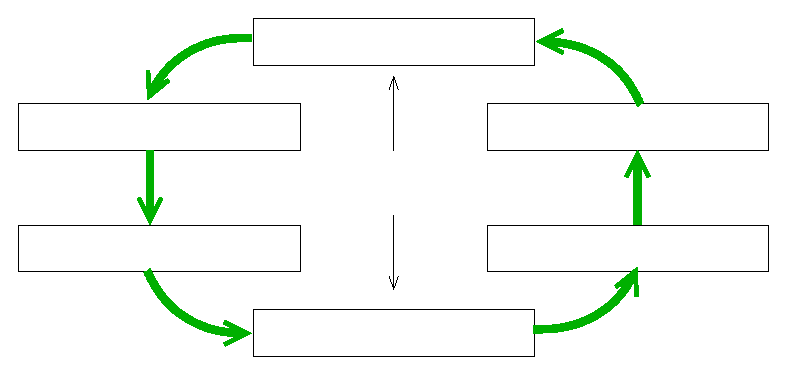
\includegraphics{getdp-magthe}%
\end{picture}%
\setlength{\unitlength}{3947sp}%
%
\begingroup\makeatletter\ifx\SetFigFont\undefined%
\gdef\SetFigFont#1#2#3#4#5{%
  \reset@font\fontsize{#1}{#2pt}%
  \fontfamily{#3}\fontseries{#4}\fontshape{#5}%
  \selectfont}%
\fi\endgroup%
\begin{picture}(6024,2724)(1489,-4723)
\put(4501,-4561){\makebox(0,0)[b]{\smash{\SetFigFont{10}{12.0}{\rmdefault}{\mddefault}{\updefault}{\color[rgb]{0,0,0}\textsf{Thermal problem}}%
}}}
\put(2626,-2911){\makebox(0,0)[b]{\smash{\SetFigFont{10}{12.0}{\rmdefault}{\mddefault}{\updefault}{\color[rgb]{0,0,0}\textsf{Joule power density}}%
}}}
\put(2701,-3886){\makebox(0,0)[b]{\smash{\SetFigFont{10}{12.0}{\rmdefault}{\mddefault}{\updefault}{\color[rgb]{0,0,0}\textsf{Thermal source density}}%
}}}
\put(4501,-3361){\makebox(0,0)[b]{\smash{\SetFigFont{10}{12.0}{\rmdefault}{\mddefault}{\updefault}{\color[rgb]{0,0,0}\textsf{Nonlinear problems}}%
}}}
\put(6376,-3886){\makebox(0,0)[b]{\smash{\SetFigFont{10}{12.0}{\rmdefault}{\mddefault}{\updefault}{\color[rgb]{0,0,0}\textsf{Temperature field}}%
}}}
\put(4501,-2236){\makebox(0,0)[b]{\smash{\SetFigFont{10}{12.0}{\rmdefault}{\mddefault}{\updefault}{\color[rgb]{0,0,0}\textsf{Magnetodynamic problem}}%
}}}
\put(6376,-2911){\makebox(0,0)[b]{\smash{\SetFigFont{10}{12.0}{\rmdefault}{\mddefault}{\updefault}{\color[rgb]{0,0,0}\textsf{Electric physical properties}}%
}}}
\end{picture}
}
\end{center}

\end{slide}

\begin{slide}

\mybox{colbox}{0.98\textwidth}{
\begin{center}
Magnetodynamic formulations
\end{center}
\begin{slideitemize}
\item Adapted function spaces for the fields and potentials involved
\item Boundary conditions
\item Electric circuit coupling, prescribed currents or voltages
\item Nonlinear magnetic characteristics
\end{slideitemize}
}

\parbox{0.1\textwidth}{e.g.}\parbox{0.9\textwidth}{
\begin{gather*}
\ivol[_{\Omega}]{\mu^{-1}\Curl{\vec{a}}}{\Curl{\vec{a}'}} +
\ivol[_{\Omega_c}]{\sigma\partial_t\vec{a}}{\vec{a}'} +
\ivol[_{\Omega_c}]{\sigma\Grad{v}}{\vec{a}'} = 
0, \\
\forall \vec{a}'\in\Hcurl[_0]{\Omega}
\end{gather*}
\begin{equation*}
\partial_t\ivol[_{\Omega}]{\mu\vec{h}}{\vec{h}'} +
\ivol[_{\Omega_c}]{\sigma^{-1}\Curl{\vec{h}}}{\Curl{\vec{h}'}} =
0, \quad
\forall \vec{h}'\in\Hcurl[_0]{\Omega}
\end{equation*}
}

\end{slide}

\begin{slide}

\mybox{colbox}{0.98\textwidth}{
\begin{center}
Thermal formulation
\end{center}
\begin{slideitemize}
\item For example temperature $T$ formulation
\item Essential boundary conditions for $T$
\item Natural boundary conditions for convection and radiation heat flows
\item Nonlinear thermal characteristics
\end{slideitemize}
}

\begin{gather*}
\ivol[_\Omega]                 {\kappa\,\Grad{T}}        {\Grad{T'}}   -
\ivol[_\Omega]             {\rho c_p\,\partial_t T}         {T'}       +
\ivol[_\Omega]                      {p_q}                   {T'}   \\ +
\isur[_{\Gamma_{\text{conv}}}]    {\eta(T-T_0)}                {T'}       +
\isur[_{\Gamma_{\text{rad}}}]{\epsilon\sigma_s(T^4-T_0^4)}  {T'}     = 0  \,, 
\quad\forall T'\in \Hone[_0]{\Omega}
\end{gather*}

% $\sigma$ is Botltzmann's constant
% $\epsilon$ is the emissivity
% $\eta$ is the convection coefficient (2.5->5)
% $T_0$ is the temperature of the materials surrounding the steel part

\end{slide}

\begin{slide}

\mybox{colbox}{0.98\textwidth}{
\begin{center}
Movement of regions
\end{center}
\begin{slideitemize}
\item Addition of transport term (e.g.\ modified Ohm's law:
$\vec{j}=\sigma(\vec{e}+\pvec{\vec{v}}{\vec{b}})$)
\end{slideitemize}
}

\parbox{0.1\textwidth}{e.g.}\parbox{0.9\textwidth}{
\begin{gather*}
-\ivol[_{\Omega_v}]{ \sigma \pvec{\vec{v}} {\Curl{\vec{a}}} } {\vec{a}'}\\
-\ivol[_{\Omega_v}]{ \mu    \pvec{\vec{v}} {\vec{h}}        } {\Curl{\vec{h}'}}
\end{gather*}
}
\parbox{0.1\textwidth}{e.g.}\parbox{0.9\textwidth}{
\begin{equation*}
-\ivol[_{\Omega_v}]{\rho c_p\psca{\vec{v}}{\Grad{T}}}{T'}
\end{equation*}
}

\end{slide}

\begin{slide}

\mybox{colbox}{0.98\textwidth}{
\begin{center}
Magneto-thermal coupling
\end{center}
\begin{slideitemize}
\item Heat source term $p_q=\frac{1}{2}\sigma^{-1}j^2$
\item Temperature dependent electric and magnetic characteristics $\mu(T)$ and
$\sigma(T)$
\end{slideitemize}
}

\parbox{0.1\textwidth}{e.g.}\parbox{0.9\textwidth}{
\begin{gather*}
j=\sigma\|\partial_t\vec{a}+\Grad{v}\|\\
j=\|\Curl{\vec{h}}\|
\end{gather*}
}

\end{slide}

\begin{slide}[1.02\slidewidth,\slideheight]

\mybox{colbox}{0.98\textwidth}{
\begin{center}
Resolutions
\end{center}
\begin{slideitemize}
\item Magnetodynamic resolution in time or frequency domain
\item Thermal resolution in steady state or in time domain
\end{slideitemize}
}

% NbrMaxIteration 16; RelaxationFactor 1; Criterion 1.e-4;
\begin{smallsyntax}
Resolution \{ \CC{magnetodynamic freq + thermal static}
  \{ Name Magnetothermal_h_T;
    System \{
      \{ Name Mag; NameOfFormulation MagDyn_h; Frequency 50; \}
      \{ Name The; NameOfFormulation The_T \}
    \}
    Operation \{
      IterativeLoop[16,1.e-4,1] \{ \CC{max_its, stop, relax}
        GenerateJac[Mag]; SolveJac[Mag]; GenerateJac[The]; SolveJac[The];
      \}
      SaveSolution[Mag]; SaveSolution[The];
    \}
  \} \}
\end{smallsyntax}

\end{slide}

% ---------------------------------------------------------------------------

\background{}{}{}

\ifnum\bigpictures=1

\chapter{Other examples...}

\begin{slide}

\begin{center}
\includegraphics[width=\textwidth]{getdp-picts/antenna1}
\includegraphics[width=\textwidth]{getdp-picts/antenna3}
\includegraphics[width=\textwidth]{getdp-picts/antenna2}
\includegraphics[height=\textheight]{getdp-picts/indheat}
\includegraphics[angle=-90,width=\textwidth]{getdp-picts/line220kv}
\includegraphics[height=\textheight]{getdp-picts/magnet}
\includegraphics[height=\textheight]{getdp-picts/motoras}

\hspace*{-0.2\textwidth}%
\includegraphics[width=0.5\textwidth]{getdp-picts/p20induc2}\hspace*{-0.2\textwidth}
\includegraphics[width=0.5\textwidth]{getdp-picts/p20}\hspace*{-0.2\textwidth}%
\includegraphics[width=0.5\textwidth]{getdp-picts/p20ada}\hspace*{-0.2\textwidth}%

Piezo-electricity, magnetostriction, non-homogeneous waveguides, photonic
cristals, electromagnetic shielding, dielectric heating, ...

\end{center}

\end{slide}

\fi

